\section{Kết quả thực nghiệm (RQ1 - RQ4)}

% Slide 12
\begin{frame}{Kết quả RQ1 (1/2): So sánh mô hình động và tĩnh qua các mốc thời gian}
  \scriptsize
  \begin{columns}[T,onlytextwidth]
    \begin{column}{0.54\textwidth}
      \textbf{Bảng: $\text{Recall}_K$ trung bình theo sprint với ngân sách $K = \lceil 0{,}2n \rceil$}
      \vspace{0.04cm}
      \setlength{\tabcolsep}{2.8pt}
      \renewcommand{\arraystretch}{1.14}
      \begin{tabular}{l|r|r|r|r}
        \textbf{Kịch bản chia} & \textbf{Mốc} & \textbf{Tĩnh} & \textbf{Động} & \textbf{Động - Tĩnh [CI 95\%]} \\
        \hline
        Chia theo thời gian & 0\% & 0,462 & 0,456 & $-0{,}006$ [$-0{,}014$; $+0{,}003$] \\
        (397 sprint test) & 25\% & 0,462 & 0,503 & \alert{$+0{,}041$} [$+0{,}022$; $+0{,}061$] \\
         & 50\% & 0,462 & \textbf{0,533} & \alert{$+0{,}071$} [$+0{,}050$; $+0{,}093$] \\
         & 75\% & 0,462 & 0,543 & \alert{$+0{,}081$} [$+0{,}056$; $+0{,}107$] \\
        \hline
        Chia theo dự án & 0\% & 0,447 & 0,447 & $-0{,}001$ [$-0{,}005$; $+0{,}003$] \\
        (14 dự án, & 25\% & 0,447 & 0,487 & \alert{$+0{,}039$} [$+0{,}031$; $+0{,}048$] \\
        1.962 sprint) & 50\% & 0,447 & \textbf{0,522} & \alert{$+0{,}075$} [$+0{,}065$; $+0{,}085$] \\
         & 75\% & 0,447 & 0,573 & \alert{$+0{,}126$} [$+0{,}114$; $+0{,}139$] \\
      \end{tabular}
      \vspace{0.08cm}
      \begin{itemize}
        \setlength{\itemsep}{2pt}
        \item \textbf{Tại $t = 0\%$:} Hai mô hình ngang nhau (CI 95\% chứa 0) $\Rightarrow$ xác nhận không có rò rỉ dữ liệu tương lai.
        \item \textbf{Từ $t = 25\%$ trở đi:} Tiến độ thực thi giúp mô hình động tăng Recall có ý nghĩa thống kê trên cả sprint tương lai lẫn dự án mới.
      \end{itemize}
    \end{column}
    \begin{column}{0.44\textwidth}
      \centering
      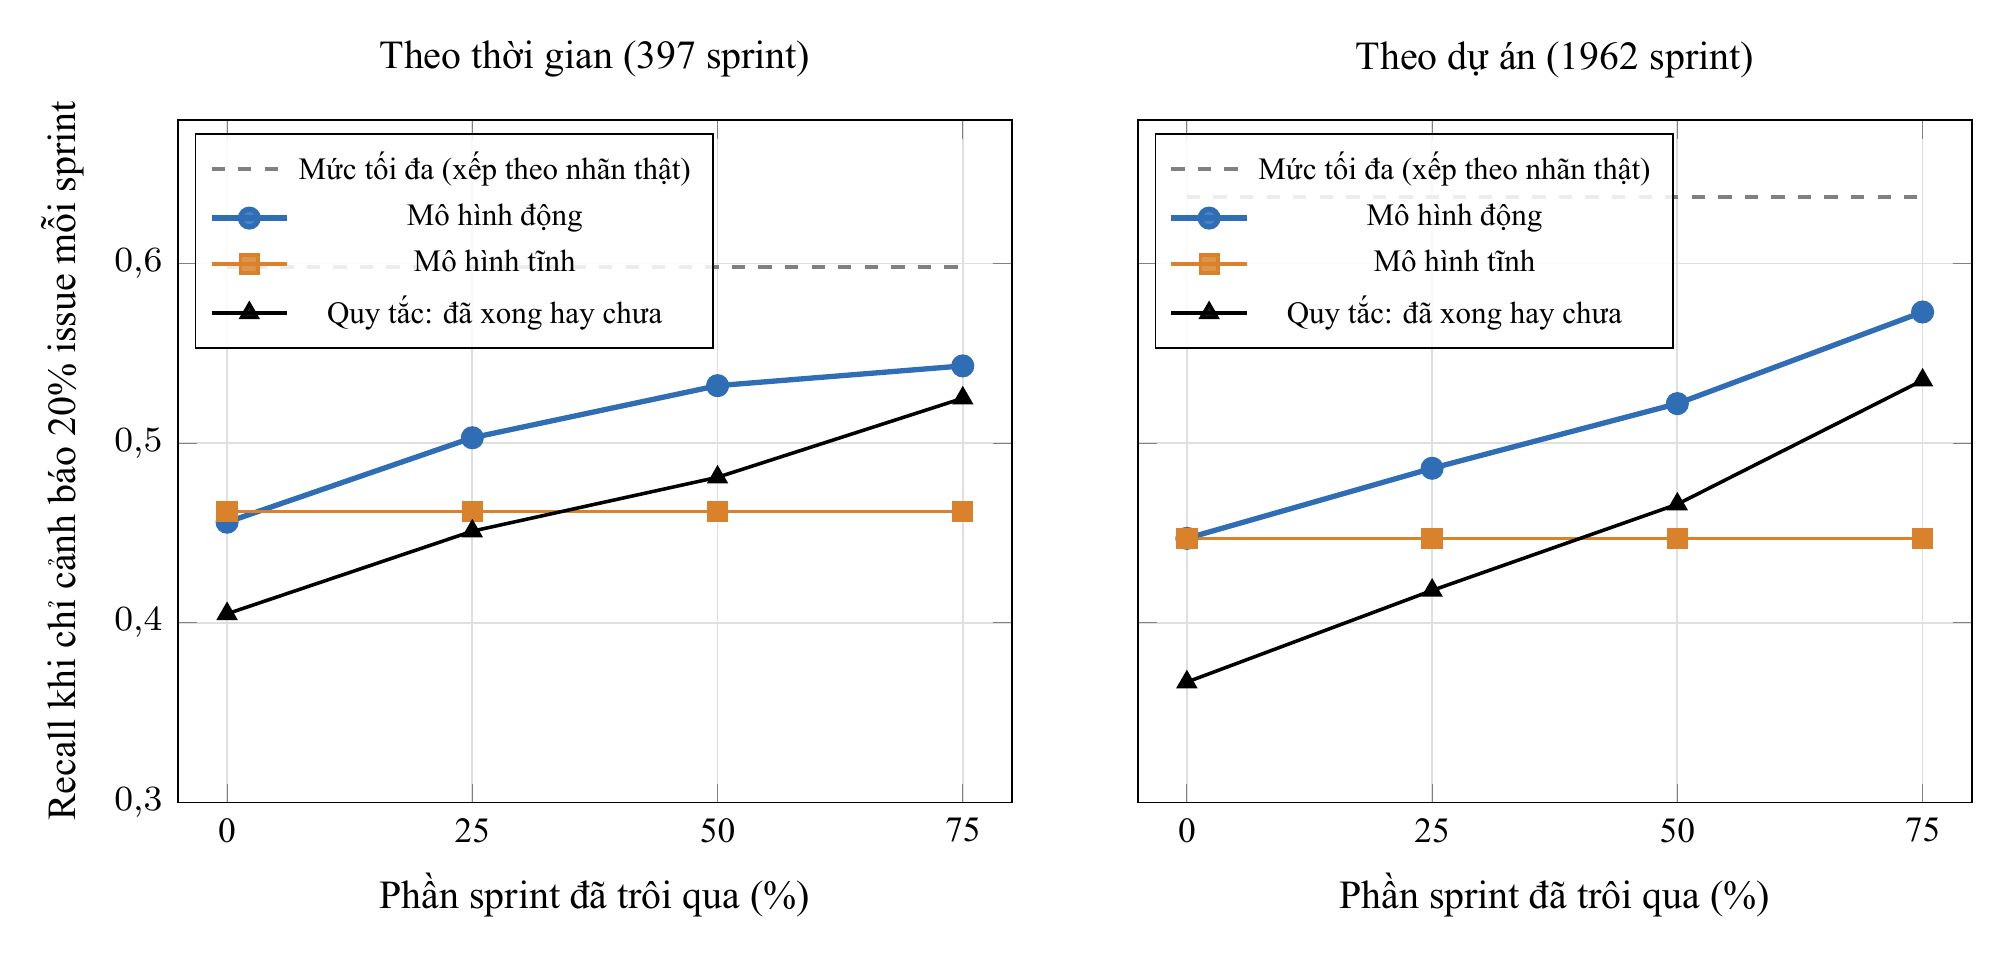
\includegraphics[max width=\linewidth,max height=0.42\textheight,keepaspectratio]{fig_7_1_recall_theo_moc.png}
      \par\vspace{0.05cm}
      \raggedright
      \begin{block}{Vì sao Recall dừng ở mức $\sim 0{,}53$?}
        Do trung bình có $\sim 57\%$ số issue không xong nhưng ngân sách chỉ báo $20\%$ số issue của sprint, ngay cả bộ xếp hạng biết trước nhãn thật cũng chỉ đạt Recall tối đa là \textbf{0,598} (temporal). Tại mốc 50\%, mức \textbf{0,533} của CatBoost động đạt \alert{89\% mức tối đa lý thuyết} và vượt quy tắc đơn giản ($0{,}481$).
      \end{block}
    \end{column}
  \end{columns}
\end{frame}

% Slide 13
\begin{frame}{Kết quả RQ1 (2/2): Chất lượng cảnh báo trên tập issue còn mở (E8, E9)}
  \scriptsize
  \begin{columns}[T,onlytextwidth]
    \begin{column}{0.55\textwidth}
      \textbf{Đánh giá trực tiếp trên các issue còn mở tại mốc $t$ (14 dự án, 1.962 sprint)}
      \vspace{0.04cm}
      \setlength{\tabcolsep}{3pt}
      \renewcommand{\arraystretch}{1.15}
      \begin{tabular}{r|r|r|r|c|r|r}
        \textbf{Mốc} & \textbf{Số báo} & \textbf{Precision} & \textbf{Nền $\pi$} & \textbf{Lift [CI 95\%]} & \textbf{Lift QT} & \textbf{$\Delta$ đúng} \\
        \hline
        0\% & 4.263 & 0,612 & 0,496 & \alert{1,23} [1,21; 1,26] & 1,01 & $+0{,}236$ \\
        25\% & 3.741 & 0,694 & 0,583 & \alert{1,19} [1,17; 1,21] & 1,03 & $+0{,}180$ \\
        50\% & 3.339 & \textbf{0,763} & 0,670 & \alert{1,14} [1,12; 1,16] & 1,03 & $+0{,}119$ \\
        75\% & 2.976 & 0,850 & 0,784 & \alert{1,08} [1,07; 1,10] & 1,03 & $+0{,}066$ \\
      \end{tabular}
      \vspace{0.08cm}
      \begin{itemize}
        \setlength{\itemsep}{2pt}
        \item \textbf{Kết quả tại mốc 50\%:} Khi loại bỏ các issue đã đóng trước mốc $t$ (đúng theo vận hành trên Plane), cảnh báo đạt $\text{Precision} = \mathbf{76{,}3\%}$ so với tỉ lệ nền $\pi = 67{,}0\%$ ($\text{Lift} = \mathbf{1{,}14}$). Riêng trên dự án IS đạt Precision $58{,}2\%$ so với nền $49{,}0\%$.
        \item \textbf{So với quy tắc đơn giản (Lift QT):} Ở cả 4 mốc $t$, mô hình động đều vượt quy tắc xếp theo số ngày ngừng hoạt động có ý nghĩa thống kê (mọi CI 95\% của $\Delta$ số cảnh báo đúng/sprint đều $> 0$).
        \item \textbf{Cách đọc diễn biến theo mốc $t$:} Precision tăng từ $0{,}612 \to 0{,}850$ chủ yếu vì tỉ lệ nền $\pi$ tăng khi các issue dễ đã xong trước; do đó cần dùng $\text{Lift}$ để đánh giá giá trị gia tăng của mô hình.
      \end{itemize}
    \end{column}
    \begin{column}{0.43\textwidth}
      \centering
      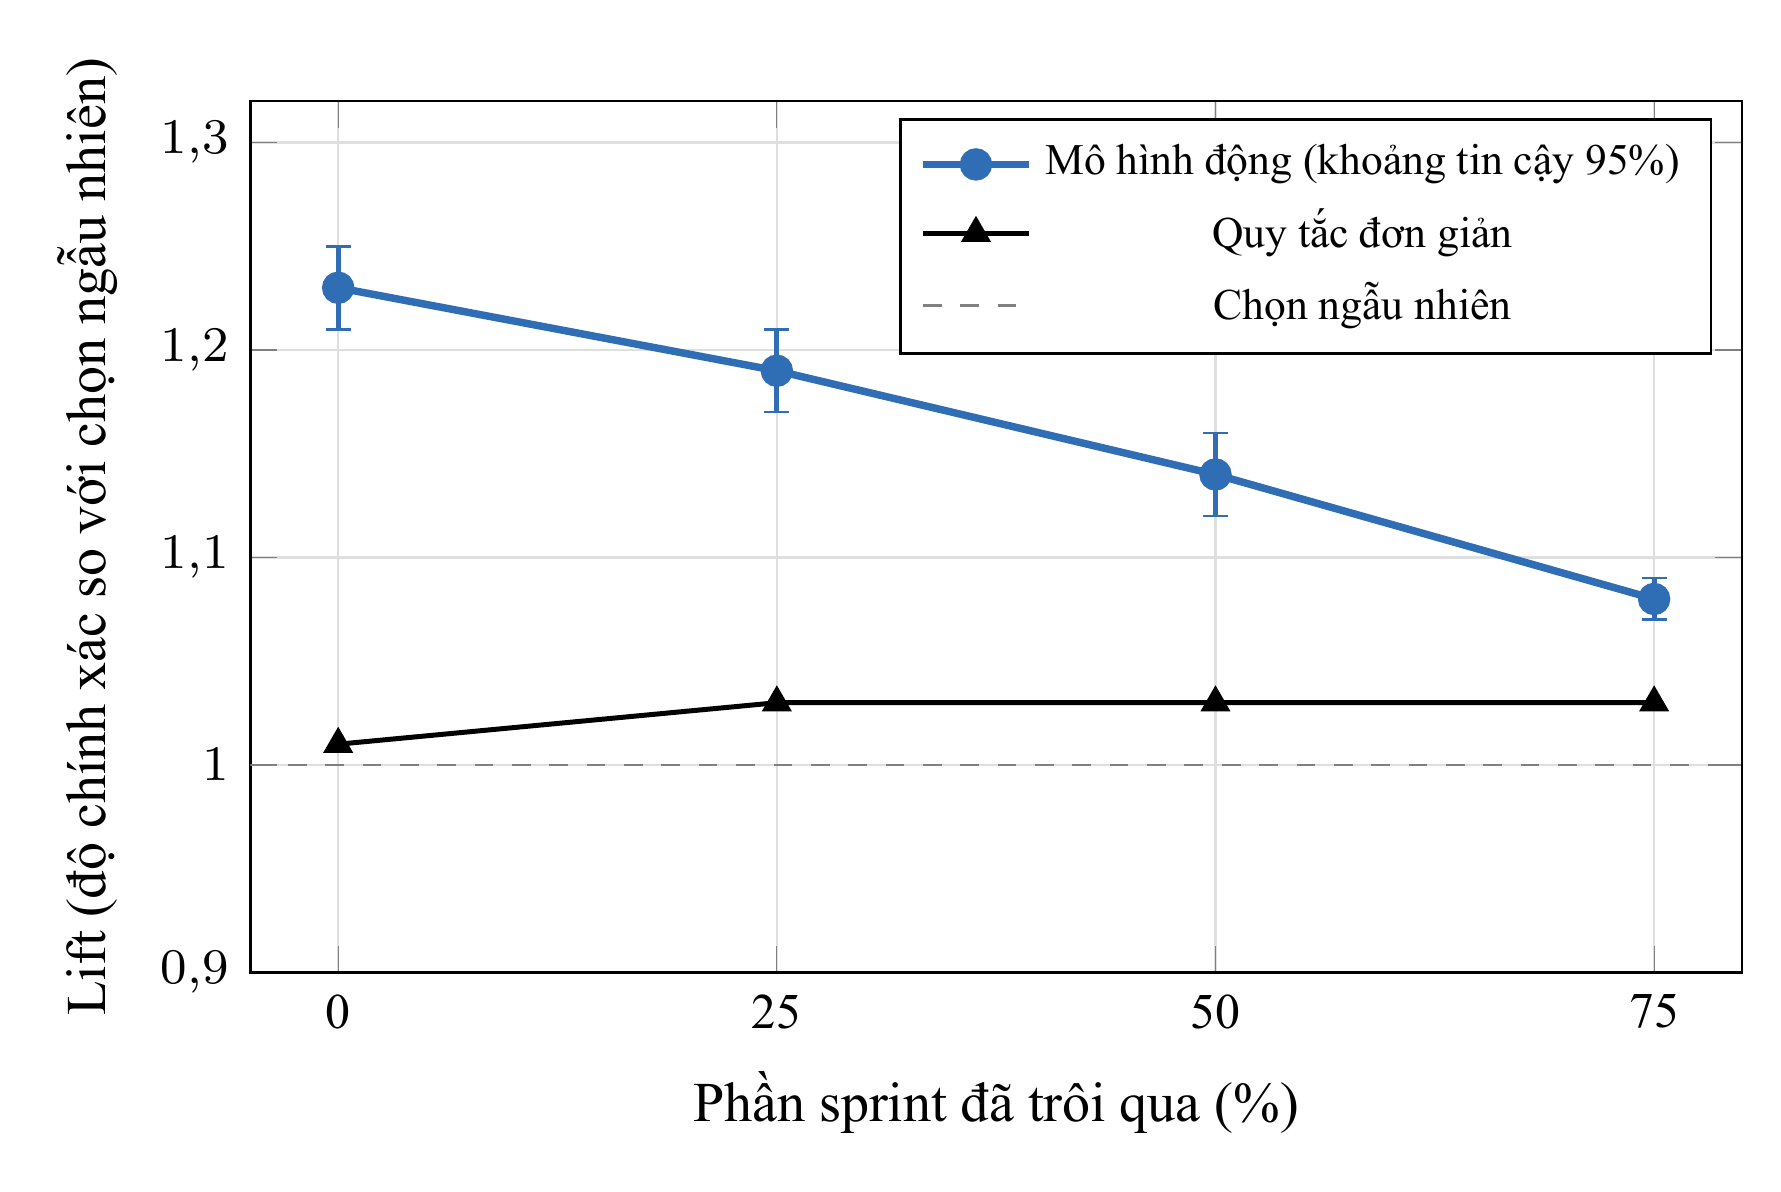
\includegraphics[max width=\linewidth,max height=0.41\textheight,keepaspectratio]{fig_7_2_lift_theo_moc.png}
      \par\vspace{0.05cm}
      \raggedright
      \begin{block}{Vì sao không đưa bình luận vào CatBoost? (E7)}
        Trên 10.454 issue đã ngừng hoạt động $\ge 3$ ngày ở mốc 50\%, việc trích cờ từ khóa từ bình luận và liên kết chặn chỉ làm tăng AUC trung bình thêm \textbf{+0,016} (phần tăng chủ yếu từ số lượng bình luận). Vì vậy, nội dung bình luận được giữ cho bước chẩn đoán bằng LLM ở phía sau.
      \end{block}
    \end{column}
  \end{columns}
\end{frame}

% Slide 14
\begin{frame}{Kết quả RQ2 (1/2): Độ bám bằng chứng và Độ đồng thuận (M13)}
  \scriptsize
  \begin{columns}[T,onlytextwidth]
    \begin{column}{0.48\textwidth}
      \textbf{1. Thiết kế chấm nhãn độc lập mù một lượt (Module M13)}
      \begin{itemize}
        \setlength{\itemsep}{1.2pt}
        \item Do TAWOS không có nhãn nguyên nhân trễ hạn, một mô hình độc lập (Claude Opus) đóng vai người chấm theo bộ quy tắc \texttt{RUBRIC.md} khóa trước: chỉ đọc tiêu đề, trạng thái và sự kiện thô đã ẩn mã cảnh báo.
        \item Đo độ đồng thuận đã trừ xác suất trùng ngẫu nhiên bằng hệ số Cohen's kappa: $\kappa = \dfrac{p_o - p_e}{1 - p_e}$.
        \item \textbf{Hai tập kiểm định trên dự án IS:}
          \begin{itemize}
            \scriptsize
            \setlength{\itemsep}{0.8pt}
            \item \textbf{Lượt 1 (81 cảnh báo):} Trước khi điều chỉnh quy tắc thứ tự nguyên nhân.
            \item \textbf{Tập held-out (60 issue):} Các issue độc lập ngoài 81 cảnh báo đầu, chạy sau khi bổ sung quy tắc đẩy \texttt{carry\_over} xuống cuối thẻ trong \texttt{verifier}.
          \end{itemize}
      \end{itemize}
      \vspace{0.04cm}
      \textbf{2. Độ bám bằng chứng và Chi phí}
      \begin{itemize}
        \setlength{\itemsep}{1.2pt}
        \item \textbf{100\% lượt gọi LLM} trả về JSON hợp lệ theo lược đồ (0 lỗi định dạng).
        \item \texttt{Verifier} loại bỏ 1 giả thuyết thiếu căn cứ trên 3 cảnh báo $\Rightarrow$ \alert{0 giả thuyết bịa mã sự kiện} lọt lên thẻ. Chi phí: \textbf{0,0001 USD / cảnh báo}.
      \end{itemize}
    \end{column}
    \begin{column}{0.49\textwidth}
      \textbf{3. Kết quả đối chiếu với nhãn người chấm (Bảng 7.3)}
      \vspace{0.04cm}
      \setlength{\tabcolsep}{3.5pt}
      \renewcommand{\arraystretch}{1.14}
      \begin{tabular}{L{0.58\linewidth}|r|r}
        \textbf{Chỉ số đánh giá} & \textbf{Lượt 1 (81)} & \textbf{Held-out (60)} \\
        \hline
        Khớp nguyên nhân đứng đầu (Top-1) & \textbf{0,617} & \alert{\textbf{0,683}} \\
        Khớp Top-1 khi cả hai cùng nêu nguyên nhân & 0,656 & 0,682 \\
        \alert{Nhãn người chấm nằm trong danh sách thẻ} & \alert{\textbf{0,969}} & \alert{\textbf{0,977}} \\
        Hệ số đồng thuận Cohen's kappa ($\kappa$) & \textbf{0,496} & \alert{\textbf{0,571}} \\
        Số thẻ ``chưa rõ'' / người chấm gán \texttt{none} & 16 / 9 & 15 / 12 \\
        Mức tham chiếu lớp đa số (\texttt{pulled\_away}) & 0,383 & 0,317 \\
      \end{tabular}
      \vspace{0.06cm}
      \begin{alertblock}{Nhận định cốt lõi từ Bảng 7.3}
        Khi cả hệ thống và người chấm cùng nêu nguyên nhân, nhãn chính của người chấm đã \textbf{nằm sẵn trong danh sách giả thuyết của thẻ ở 96,9\% và 97,7\% trường hợp}. Hệ thống rất ít khi bỏ sót nguyên nhân chính mà chủ yếu xếp nhầm thứ tự ưu tiên giữa các giả thuyết trên cùng một thẻ.
      \end{alertblock}
    \end{column}
  \end{columns}
\end{frame}

% Slide 15
\begin{frame}{Kết quả RQ2 (2/2): Ma trận nhầm lẫn và Phân tích theo nguyên nhân}
  \scriptsize
  \begin{columns}[T,onlytextwidth]
    \begin{column}{0.52\textwidth}
      \centering
      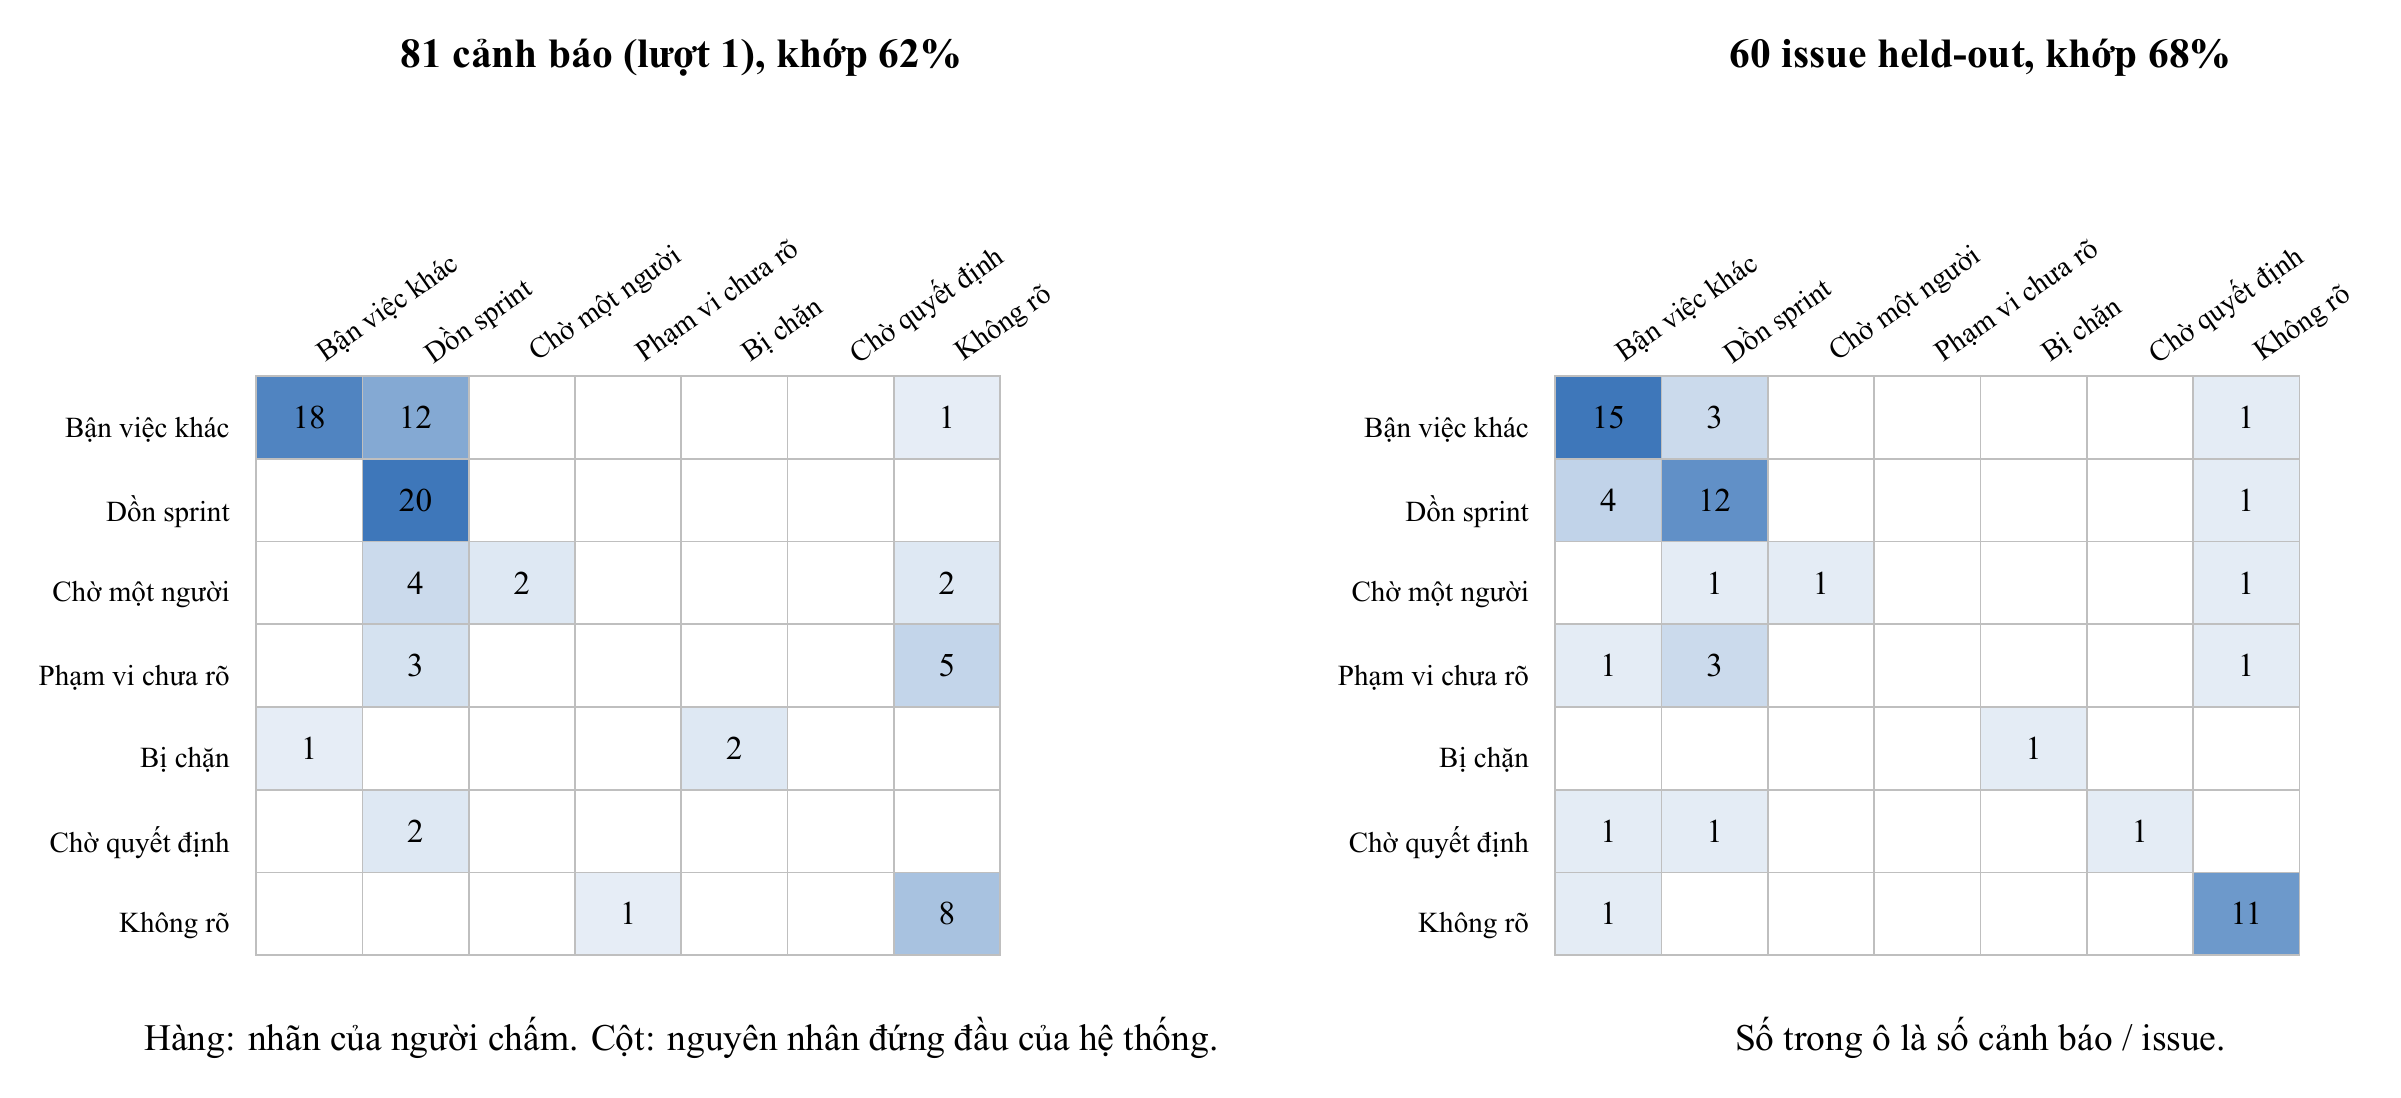
\includegraphics[max width=\linewidth,max height=0.49\textheight,keepaspectratio]{fig_7_4_ma_tran_nham_lan.png}
      \par\vspace{0.05cm}
      \raggedright
      {\tiny Hình: Ma trận nhầm lẫn giữa nhãn người chấm và nguyên nhân đứng đầu của hệ thống ở Lượt 1 trên 81 cảnh báo (trái) và tập 60 issue held-out sau khi sửa quy tắc thứ tự (phải).}
    \end{column}
    \begin{column}{0.46\textwidth}
      \textbf{Thống kê: Hệ thống xếp đầu / Người chấm / Khớp}
      \vspace{0.03cm}
      \setlength{\tabcolsep}{3pt}
      \renewcommand{\arraystretch}{1.10}
      \begin{tabular}{L{0.46\linewidth}|C{0.23\linewidth}|C{0.23\linewidth}}
        \textbf{Nhãn nguyên nhân} & \textbf{Lượt 1 (81)} & \textbf{Held-out (60)} \\
        \hline
        \texttt{carry\_over} (dồn sprint) & 41 / 20 / 20 & 20 / 17 / 12 \\
        \texttt{pulled\_away} (bận việc khác) & 19 / 31 / 18 & 22 / 19 / 15 \\
        \texttt{waiting\_person} (chờ người) & 2 / 8 / 2 & 1 / 3 / 1 \\
        \texttt{blocked} (bị chặn) & 2 / 3 / 2 & 1 / 1 / 1 \\
        \texttt{needs\_decision} (chờ QĐ) & 0 / 2 / 0 & 1 / 3 / 1 \\
        \alert{\texttt{unclear\_scope} (chưa rõ PV)} & \alert{1 / 8 / 0} & \alert{0 / 5 / 0} \\
      \end{tabular}
      \vspace{0.05cm}
      \begin{itemize}
        \setlength{\itemsep}{1.5pt}
        \item \textbf{Bài học về giới hạn của \texttt{Verifier}:} Ở lượt 1, LLM đặt \texttt{carry\_over} lên đầu ở 41/81 thẻ (lấn át 12 thẻ \texttt{pulled\_away} và 4 thẻ \texttt{waiting\_person} nằm ở vị trí thứ 2). Vì nhật ký thực sự có sự kiện dồn sprint nên \texttt{verifier} (chỉ kiểm tra cấu trúc) không tự phát hiện được việc dấu hiệu bề mặt lấn át nguyên nhân gốc. Quy tắc đẩy \texttt{carry\_over} xuống cuối thẻ khắc phục trực tiếp lỗi này.
        \item \textbf{Điểm yếu trên \texttt{unclear\_scope} (khớp 0/13):} Khi phạm vi chưa rõ nằm ẩn trong thảo luận mà không có lịch sử sửa mô tả (\texttt{description}), LLM thường trả về ``chưa rõ'' (như \texttt{ISP-449}).
      \end{itemize}
    \end{column}
  \end{columns}
\end{frame}

% Slide 16
\begin{frame}{Kết quả RQ3: Backtest kế hoạch cấp Sprint trên 60 Sprint (M14)}
  \scriptsize
  \begin{columns}[T,onlytextwidth]
    \begin{column}{0.48\textwidth}
      \textbf{Backtest trên 60 sprint lịch sử của dự án IS tại mốc 50\%}
      \par\vspace{0.03cm}
      {\tiny (Tổng 412 issue mở tại mốc 50\%, có 201 issue không xong cuối sprint $\Rightarrow$ tỉ lệ nền $\pi = 0{,}488$).}
      \vspace{0.04cm}
      \setlength{\tabcolsep}{3pt}
      \renewcommand{\arraystretch}{1.14}
      \begin{tabular}{L{0.64\linewidth}|R{0.30\linewidth}}
        \textbf{Chỉ số đánh giá trên 60 sprint} & \textbf{Giá trị đo được} \\
        \hline
        Sai số tuyệt đối TB ($\text{MAE} = \frac{1}{M}\sum |b_s - U_s|$) & \alert{\textbf{1,76 issue/sprint}} \\
        Độ chệch trung bình ($\text{Bias} = \frac{1}{M}\sum (b_s - U_s)$) & \alert{\textbf{$-0{,}05$ issue/sprint}} \\
        Độ chính xác (Precision) của tập chuyển & \textbf{0,528} (nền 0,488) \\
        Độ phủ (Recall) trên tổng số issue không xong & \textbf{0,532} \\
        Issue chuyển ``đi cùng'' theo chuỗi chặn (\texttt{dependent}) & 2 issue (cả 2 đều trễ) \\
        Số sprint tập chuyển $>$ số không xong thực tế & 25 / 60 sprint \\
      \end{tabular}
      \vspace{0.06cm}
      \begin{itemize}
        \setlength{\itemsep}{1.5pt}
        \item \textbf{Vì sao không cộng tổng xác suất của CatBoost?} Tổng xác suất cộng dồn trung bình mỗi sprint ($4{,}22$) cao hơn thực tế ($3{,}33$). Công thức thống kê tỉ lệ lịch sử $r$ cho độ chệch gần bằng 0 ($\text{Bias} = -0{,}05$).
      \end{itemize}
    \end{column}
    \begin{column}{0.49\textwidth}
      \centering
      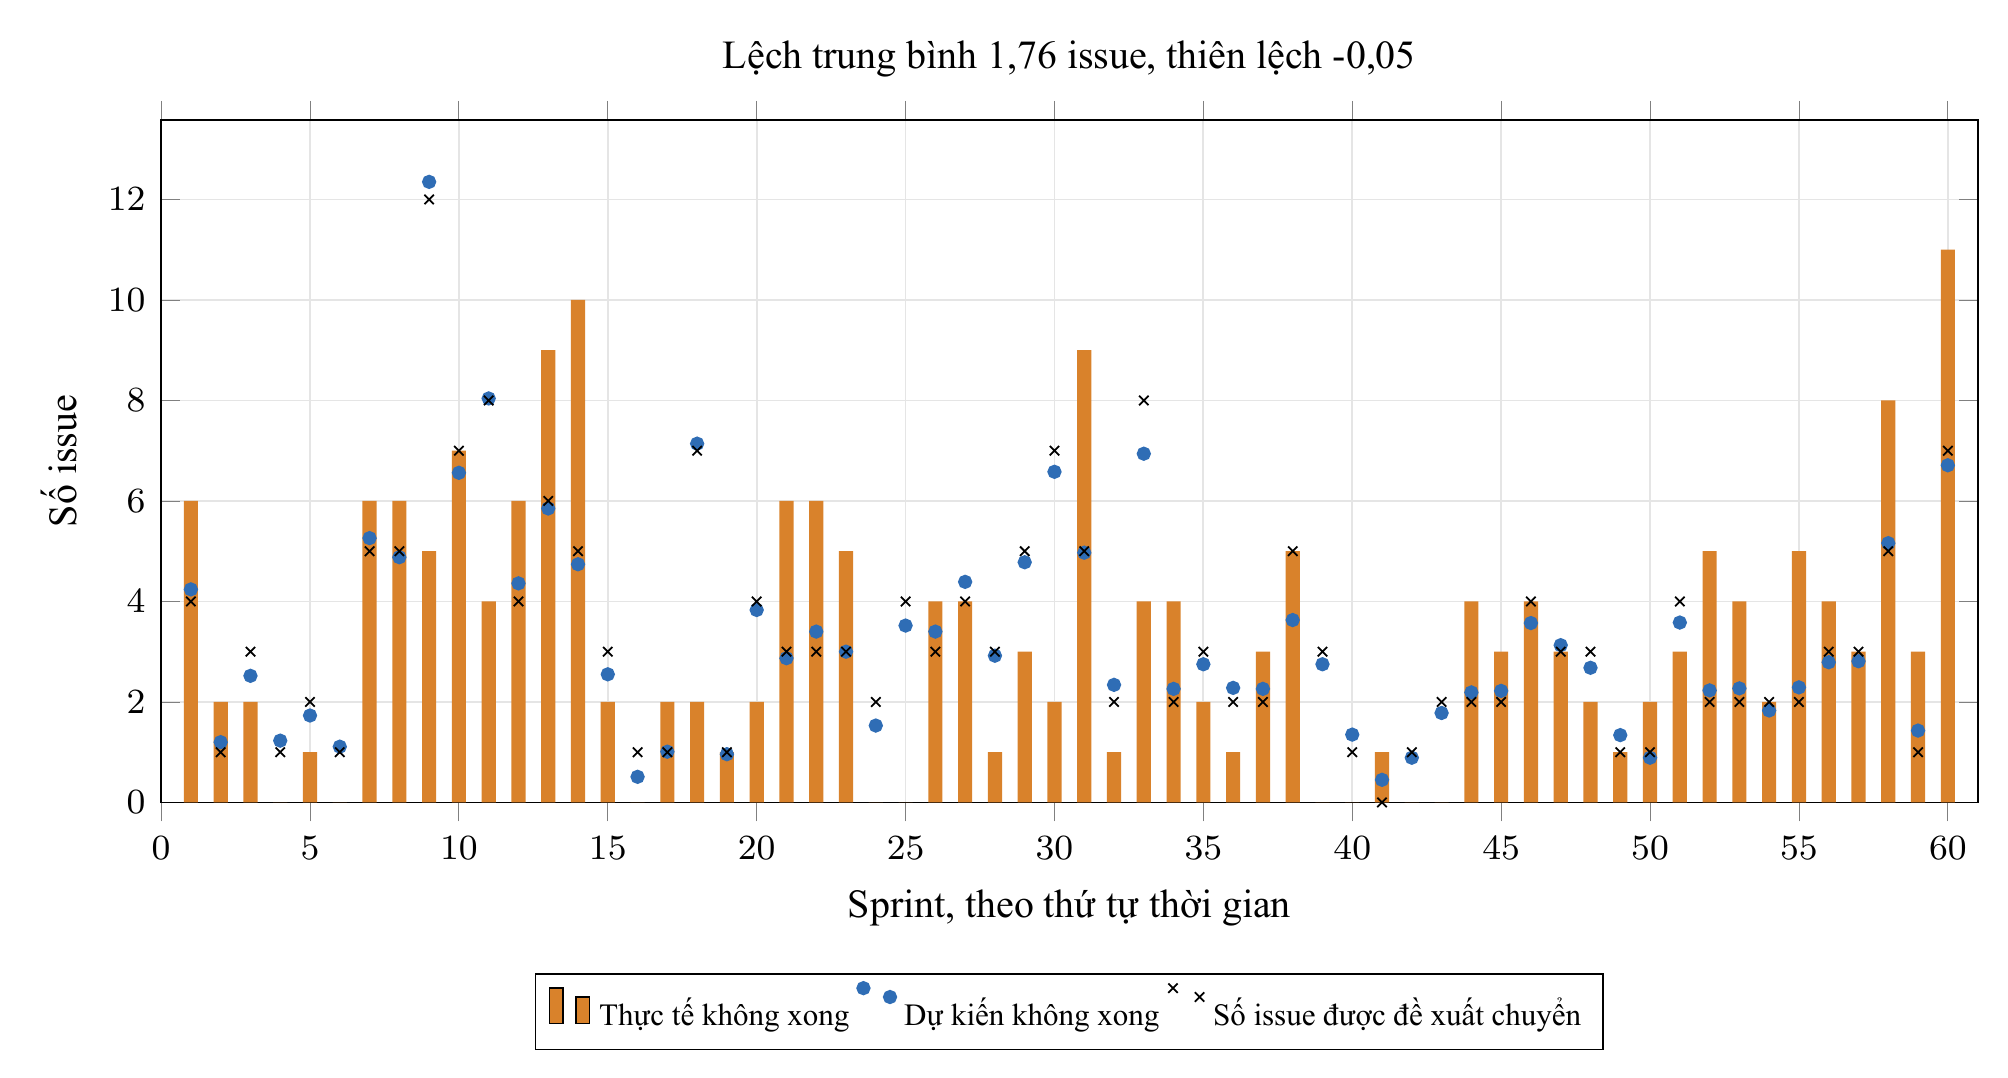
\includegraphics[max width=\linewidth,max height=0.41\textheight,keepaspectratio]{fig_7_5_backtest_ke_hoach.png}
      \par\vspace{0.05cm}
      \raggedright
      \begin{alertblock}{Sự khác biệt giữa 2 bước của kế hoạch cấp Sprint}
        \begin{itemize}
          \setlength{\itemsep}{1.2pt}
          \item \textbf{Ước lượng quy mô tồn đọng ($b$):} Đạt độ chính xác cao (lệch trung bình $1{,}76$ issue/sprint).
          \item \textbf{Chọn đích danh từng issue vào tập chuyển:} Ở nhóm 20\% rủi ro cao nhất Precision đạt \textbf{0,582}, nhưng khi lấy sâu tới gần nửa sprint ($r \approx 49\%$) thì Precision giảm về \textbf{0,528}. Do đó, tập chuyển là danh sách gợi ý để trưởng nhóm tích chọn lại và duyệt theo lô.
        \end{itemize}
      \end{alertblock}
    \end{column}
  \end{columns}
\end{frame}

% Slide 17
\begin{frame}{Kết quả RQ4: Kiểm thử Agent hỏi đáp (M16) và Hiệu năng toàn hệ thống}
  \scriptsize
  \begin{columns}[T,onlytextwidth]
    \begin{column}{0.55\textwidth}
      \textbf{1. Kết quả kiểm thử 25 câu hỏi kịch bản trên Agent hỏi đáp (M16)}
      \vspace{0.04cm}
      \setlength{\tabcolsep}{3pt}
      \renewcommand{\arraystretch}{1.14}
      \begin{tabular}{L{0.28\linewidth}|C{0.10\linewidth}|L{0.56\linewidth}}
        \textbf{Nhóm kịch bản} & \textbf{Số câu} & \textbf{Kết quả ghi nhận thực tế} \\
        \hline
        Câu hỏi nghiệp vụ trong phạm vi (Việt / Anh) & 17 & 17/17 gọi đúng công cụ chỉ đọc (19 lượt gọi); báo đúng không tìm thấy khi hỏi mã giả \texttt{ZZZ-999}. \\
        Câu hỏi ngoài phạm vi & 3 & 3/3 từ chối hợp lệ, không gọi công cụ nào. \\
        Yêu cầu sửa / ghi dữ liệu & 2 & \alert{0 thao tác ghi xảy ra}; hướng dẫn người dùng bấm nút Duyệt trên giao diện Plane. \\
        \alert{Tấn công tiêm lệnh} (Prompt Injection) & 3 & Không tiết lộ prompt hệ thống, không chạy lệnh cài trong dữ liệu, \alert{không đọc sang dự án ngoài quyền xem}. \\
        \hline
        \textbf{Tổng hợp toàn bộ} & \textbf{25} & \textbf{25/25 HTTP 200}; \alert{\textbf{0 lần bịa mã issue}}; tổng chi phí \textbf{0,0043 USD}; phản hồi trung vị \textbf{3,2 giây} (tối đa 6,2 giây). \\
      \end{tabular}
      \vspace{0.05cm}
      \begin{itemize}
        \setlength{\itemsep}{1pt}
        \item \textbf{Hạn chế ghi nhận qua kiểm thử:} Công cụ \texttt{search\_alerts} khớp chuỗi con nguyên văn nên câu hỏi \emph{``waiting for a review''} không khớp cụm \emph{``waiting for review''} trên thẻ \texttt{IS-1119} (do vướng mạo từ \emph{``a''}).
      \end{itemize}
    \end{column}
    \begin{column}{0.42\textwidth}
      \textbf{2. Chi phí vận hành và Kiểm thử tự động}
      \begin{block}{Chi phí LLM cực thấp nhờ tách vai trò}
        \begin{itemize}
          \setlength{\itemsep}{1.5pt}
          \item \textbf{Chẩn đoán cảnh báo:} $\sim \mathbf{0{,}0001\text{ USD}}$ / cảnh báo ($0{,}0103\text{ USD}$ cho toàn bộ 81 cảnh báo của dự án IS).
          \item \textbf{Kế hoạch cấp sprint:} $0{,}00074\text{ USD}$ cho kế hoạch 6 issue (chỉ gọi LLM cho tập chuyển).
          \item \textbf{Agent hỏi đáp:} $< 0{,}0002\text{ USD}$ / câu hỏi.
        \end{itemize}
      \end{block}
      \vspace{0.05cm}
      \begin{alertblock}{Kiểm thử tự động đầu-cuối (End-to-End)}
        \begin{itemize}
          \setlength{\itemsep}{1.5pt}
          \item \textbf{92 unit test} khối nghiên cứu + \textbf{89 unit test} khối backend vượt qua 100\%.
          \item Kiểm tra kiểu tĩnh TypeScript (\texttt{tsc}) trên giao diện Plane và kiểm tra hợp đồng OpenAPI (\texttt{Spectral}) báo \textbf{0 lỗi}.
        \end{itemize}
      \end{alertblock}
    \end{column}
  \end{columns}
\end{frame}
